\section{Eenvoudige thermodynamische systemen}
\subsection{PV-diagrammen (zuivere stof)}
\begin{figure}[htp]
    \centering
    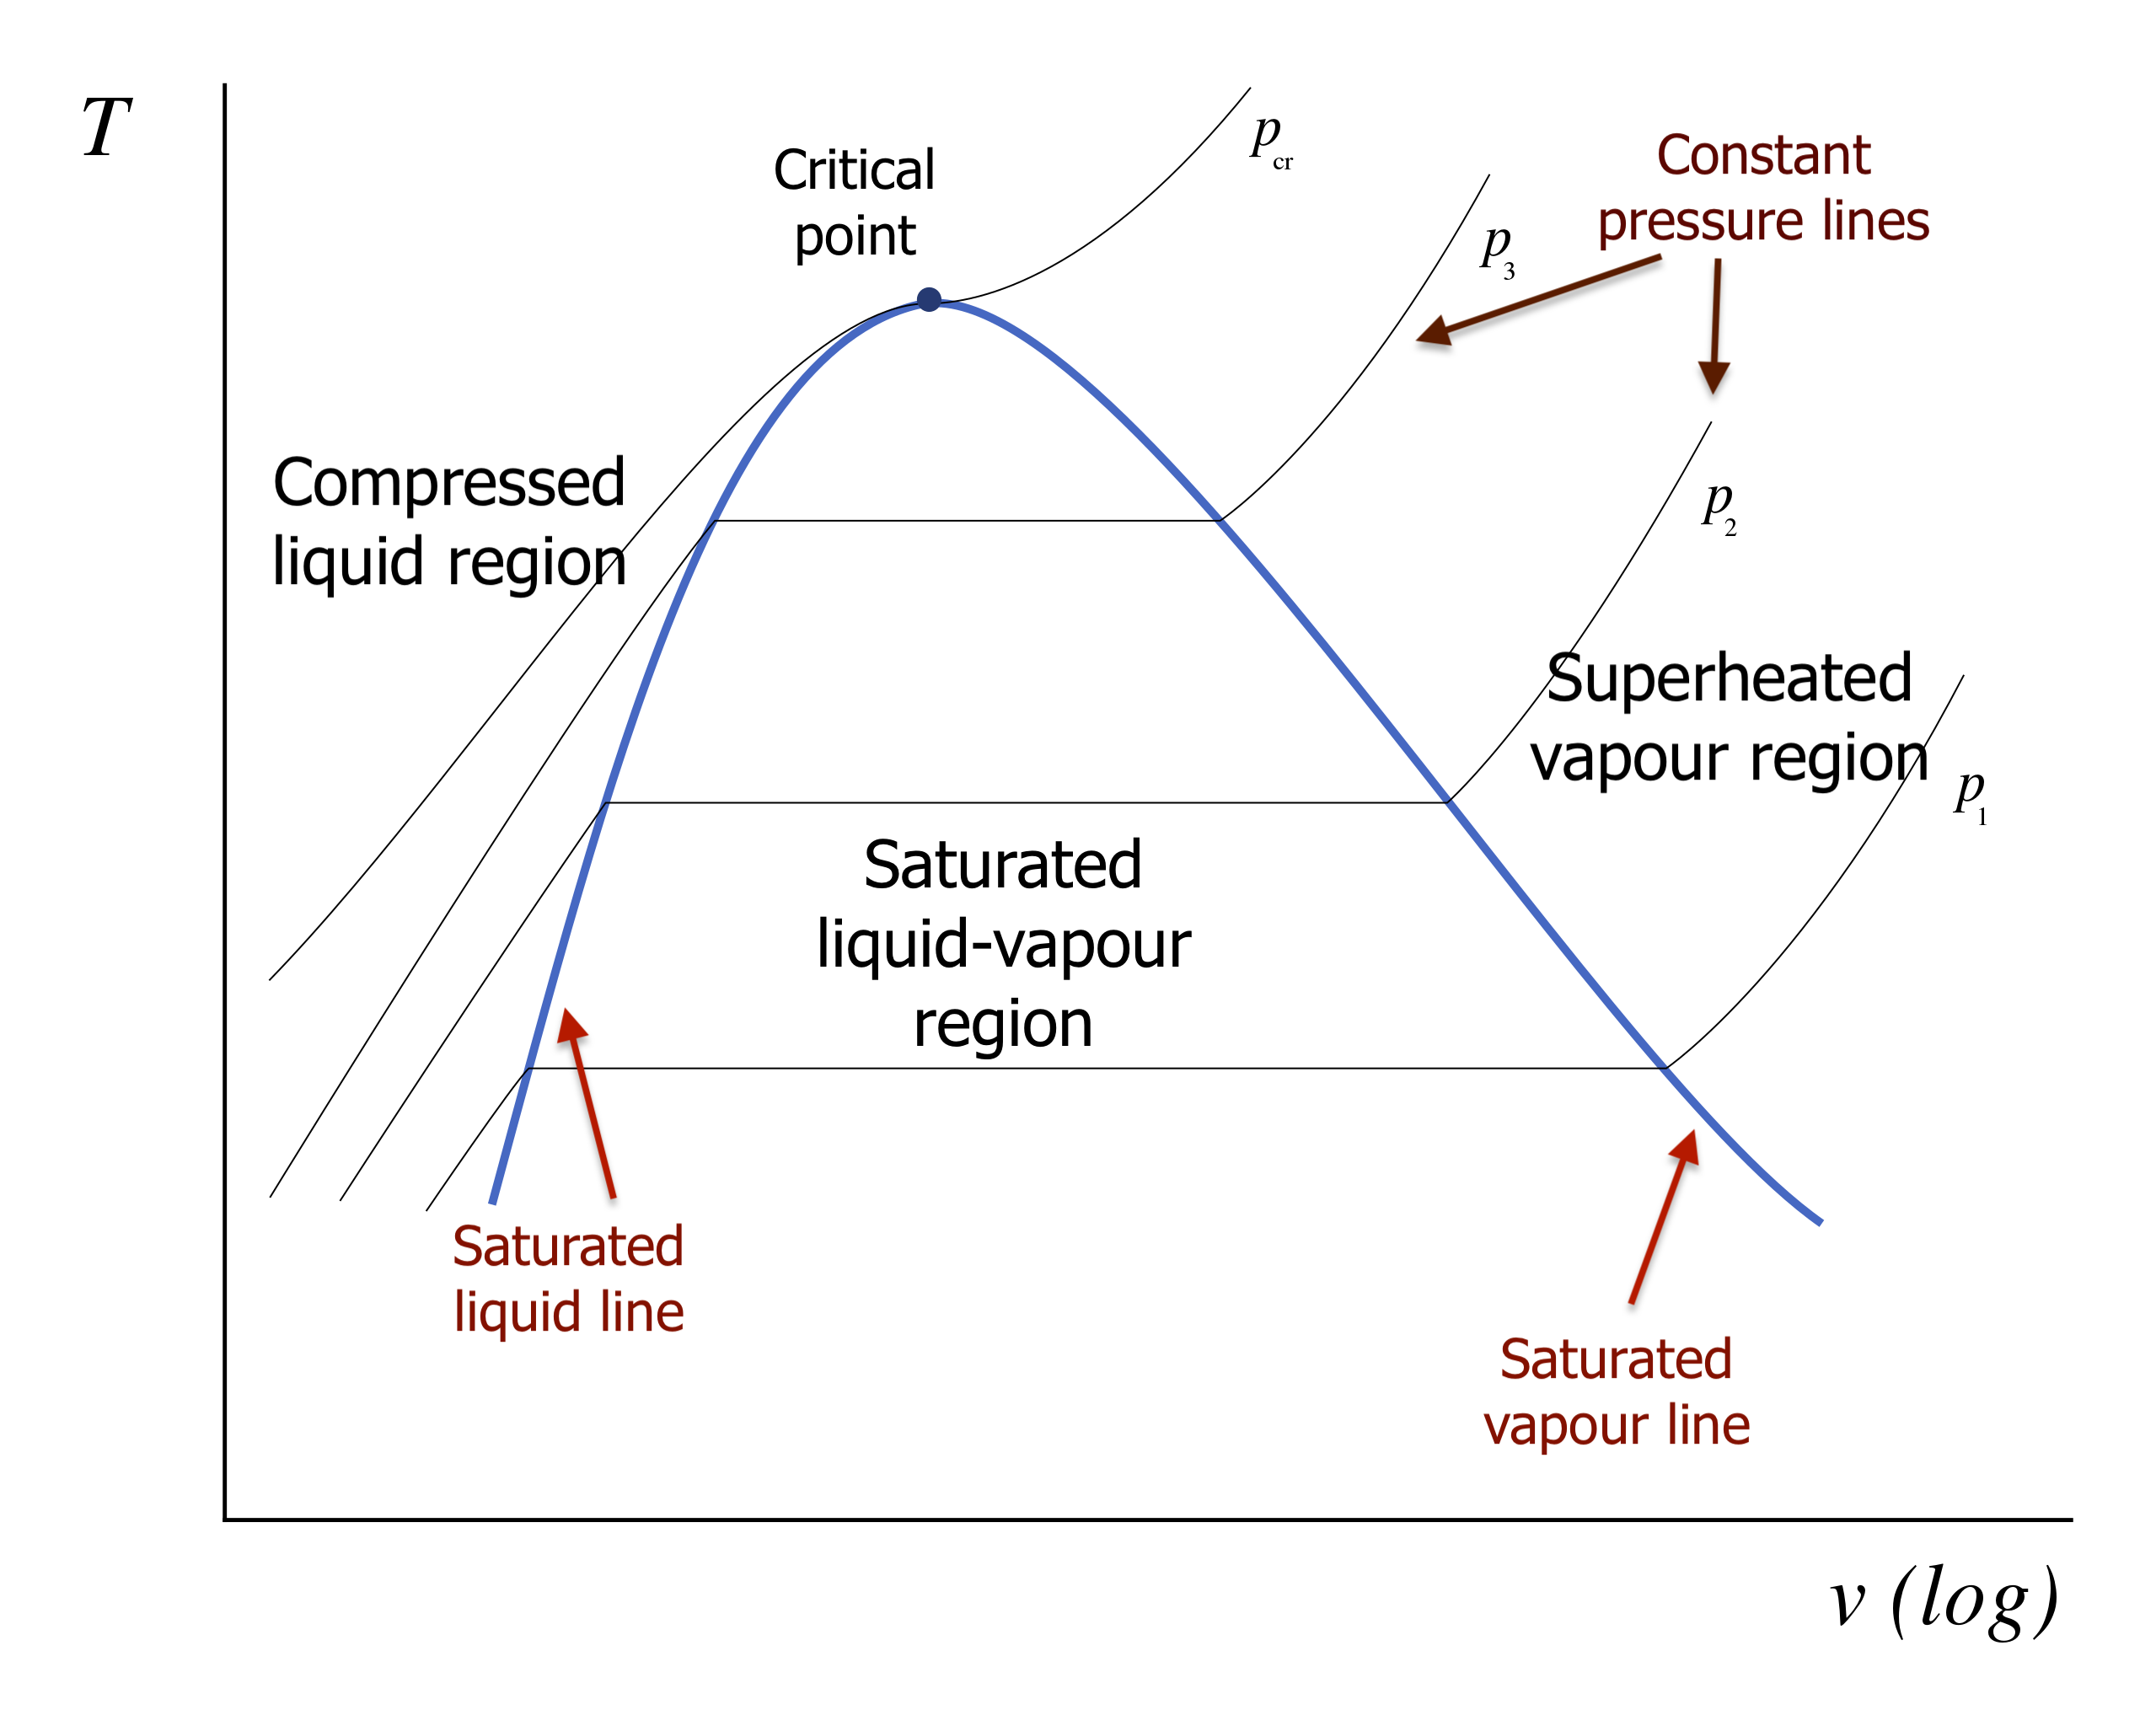
\includegraphics[width=0.5\textwidth]{Foto's-Figuren/Fig.-2-8_T-v_diagram_for_a_liquid_vapor-copy.svg_.png}
    \caption{VT-diagram van een zuivere stof. De verschillende lijnen en gebieden geven de verschillende fasen en evenwichten aan. \footnotesize \copyright{Olivier Cleynen is licensed under a CC0 (Creative Commons Zero) license}}
    \label{fig:VT-diagram}
\end{figure}
\begin{figure}
    \centering
    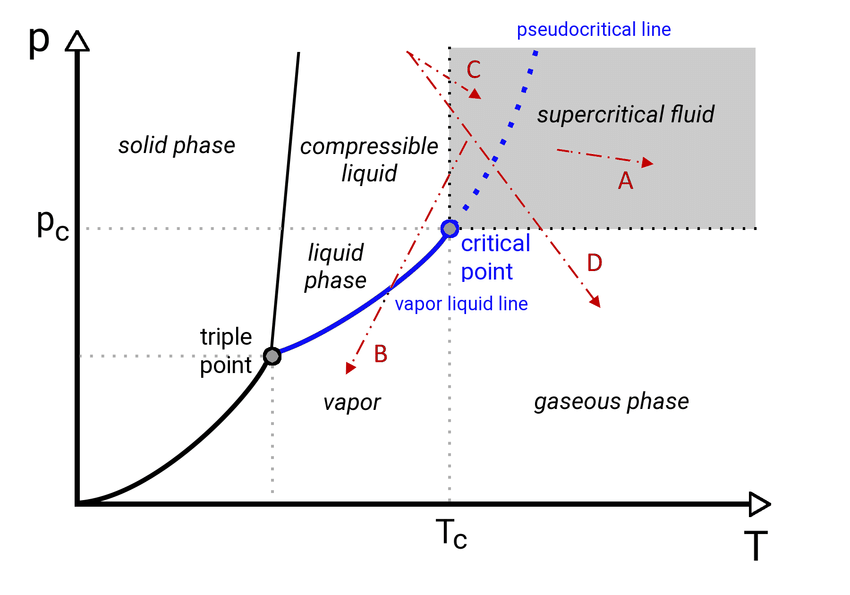
\includegraphics[width=0.5\textwidth]{Foto's-Figuren/P-T-diagram-Supercritical-fluid-region-and-various-supercritical-injection-types.ppm.png}
    \caption{PT-diagram van een zuivere stof. De verschillende lijnen en gebieden geven de verschillende fasen en evenwichten aan 
        \footnotesize \textcopyright{SUPERCRITICAL AND TRANSCRITICAL TURBULENT INJECTION PROCESSES: CONSISTENCY OF NUMERICAL MODELING - Scientific Figure on ResearchGate. Available from: \url{https://www.researchgate.net/figure/P-T-diagram-Supercritical-fluid-region-and-various-supercritical-injection-types_fig1_349274264} [accessed 10 May 2026]}}
    \label{fig:PT-diagram}
\end{figure}

\begin{figure}
    \centering
    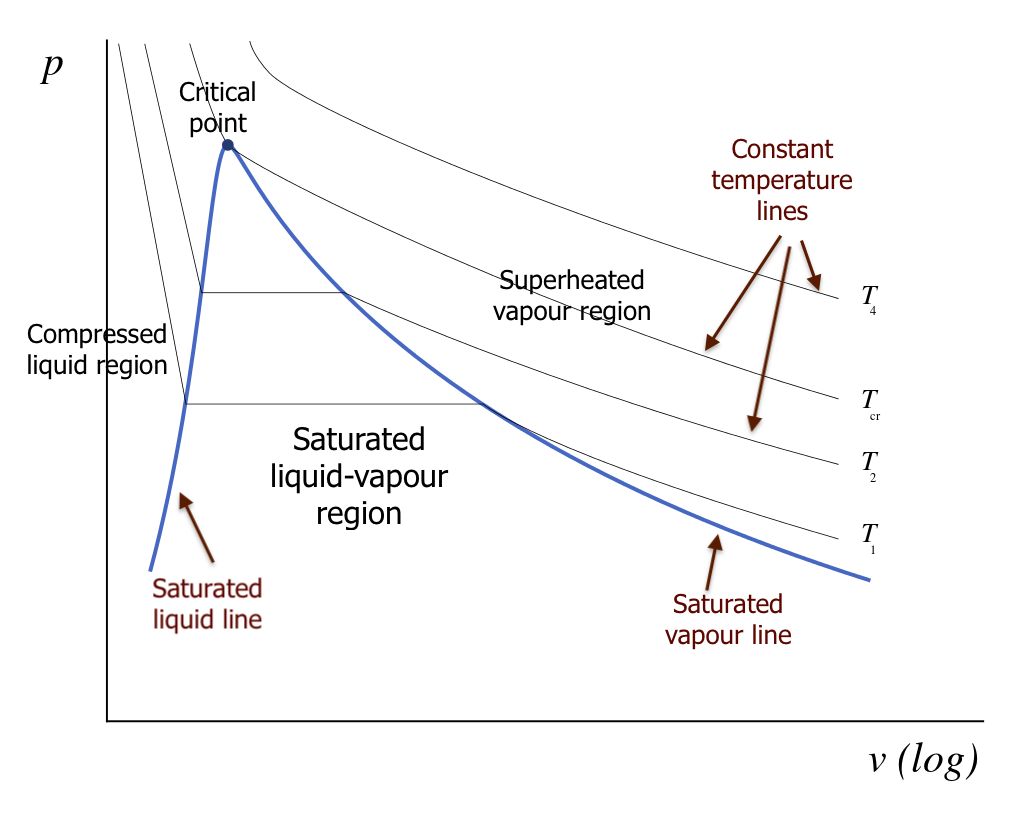
\includegraphics[width=0.5\textwidth]{Foto's-Figuren/Fig-2-9_P-v_diagram_for_a_liquid-vapor.svg_.png}
    \caption{PV-diagram van water. De verschillende lijnen en gebieden geven de verschillende fasen en evenwichten aan. \footnotesize \copyright{Olivier Cleynen is licensed under a CC0 (Creative Commons Zero) license}}
    \label{fig:PV-diagram}
\end{figure}

\begin{definition}
    \textbf{Vloeistofverzadigingslijn}: De lijn in een PV-diagram waarbij vloeistof en damp in evenwicht zijn. Deze lijn scheidt het gebied van de vloeistoftoestanden van het gebied van de damp-toestanden.
\end{definition}
\medskip
\begin{definition}
    \textbf{Kritische temperatuur}: De temperatuur waarbij de vloeistofverzadigingslijn eindigt. Boven deze temperatuur kunnen vloeistof en damp niet meer in evenwicht zijn, en is er geen onderscheid meer tussen de twee fasen.
\end{definition}
\medskip
\begin{definition}
    \textbf{Kritische isotherm}: De isotherm die door het kritische punt gaat. Deze isotherm heeft een horizontaal inflectiepunt bij het kritische punt, wat betekent dat de eerste en tweede afgeleide van de druk naar het volume gelijk zijn aan nul op dat punt.
\end{definition}
\medskip
\begin{definition}
    \textbf{Kritisch punt K}: Het punt in het PV-diagram waar de vloeistofverzadigingslijn eindigt. Op dit punt zijn de eigenschappen van de vloeistof en de damp identiek, en er is geen onderscheid meer tussen de twee fasen.
\end{definition}
\medskip
\begin{definition}
    \textbf{Kritische druk}: De druk die overeenkomt met het kritische punt in het PV-diagram. Dit is de druk waarbij de vloeistofverzadigingslijn eindigt en de kritische isotherm een horizontaal inflectiepunt heeft.
\end{definition}
\medskip
\begin{definition}
    \textbf{Verzadigde vloeistof}: Een vloeistof die in evenwicht is met haar eigen damp. Deze vloeistof heeft een constante druk en temperatuur.
\end{definition}
\medskip
\begin{definition}
    \textbf{Verzadigde damp}: Een damp die in evenwicht is met zijn eigen vloeistof. Deze damp heeft een constante druk en temperatuur.
\end{definition}
\medskip
\begin{definition}
    \textbf{Dampverzadigingslijn}: De lijn in een PV-diagram waarbij damp en vloeistof in evenwicht zijn. Deze lijn scheidt het gebied van de damp-toestanden van het gebied van de vloeistoftoestanden.
\end{definition}
\medskip
De dampverzadigingslijn en de vloeistofverzadigingslijn ontmoeten elkaar bij het kritische punt K, waar de eigenschappen van de vloeistof en de damp identiek zijn.

\begin{definition}
    \textbf{Tripellijn}: De lijn in een PV-diagram waarbij de vloeistof-damp en vaste-stof-damp in evenwicht zijn. (Dus nog niet perse de vloeibare fase inbegrepen)
\end{definition}
\subsection{PT-diagrammen (zuivere stof)}
\begin{definition}
    \textbf{Tripelpunt}: Het punt in een PV(T)-diagram waar de drie fasen van een stof in evenwicht zijn. Op dit punt kunnen alle drie de fasen tegelijkertijd bestaan. Dit punt ligt op de tripellijn van het Pv-diagram.
\end{definition}
\medskip
\begin{definition}
    \textbf{Sublimatielijn}: De lijn in een PT-diagram waarbij de vaste stof en de damp in evenwicht zijn. Deze lijn scheidt het gebied van de vaste-stof-toestanden van het gebied van de damp-toestanden.
\end{definition}
\medskip
\begin{definition}
    \textbf{Verdampingslijn}: De lijn in een PT-diagram waarbij de vloeistof en de damp in evenwicht zijn. Deze lijn scheidt het gebied van de vloeistoftoestanden van het gebied van de damp-toestanden.
\end{definition}
\medskip
\begin{definition}
    \textbf{Stollingslijn}: De lijn in een PT-diagram waarbij de vaste stof en de vloeistof in evenwicht zijn. Deze lijn scheidt het gebied van de vaste-stof-toestanden van het gebied van de vloeistoftoestanden.
\end{definition}
De drie scheidingslijnen (sublimatielijn, verdampingslijn en stollingslijn) ontmoeten elkaar bij het tripelpunt, waar alle drie de fasen in evenwicht zijn.
De helling van de sublimatielijn en verdampingslijn is altijd positief, terwijl de helling van de stollingslijn kan variëren afhankelijk van de stof.
Voor water heeft de stollingslijn een negatieve helling, wat betekent dat de smelttemperatuur van water afneemt met toenemende druk.
Voor de meeste andere stoffen heeft de stollingslijn een positieve helling, wat betekent dat de smelttemperatuur toeneemt met toenemende druk.

\subsection{Het PVT-opprevlak}
Het is belangrijk dat je deze 3D diagrammen goed kan interpreteren, en dat je weet wat de verschillende lijnen en vlakken betekenen en ze kan uitleggeen aan de hand van voorgaande definities.

\begin{figure}[h]
    \centering
    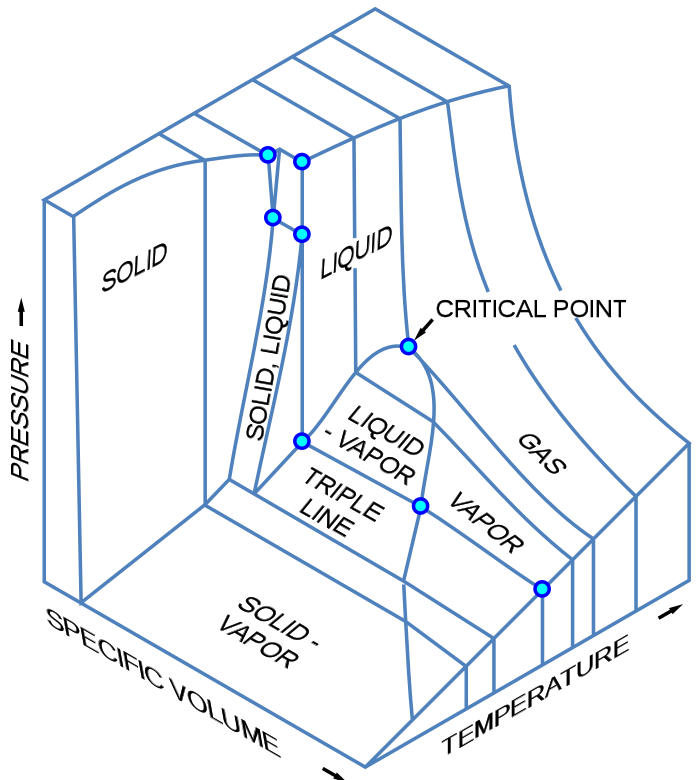
\includegraphics[width=0.5\textwidth]{Foto's-Figuren/Fig.-2-6-1.png}
    \caption{PVT-diagram van een zuivere stof. De verschillende lijnen en gebieden geven de verschillende fasen en evenwichten aan.\footnotesize \copyright{ vectorization is licensed under a CC0 (Creative Commons Zero) license.}}
    \label{fig:PVT-diagram}
\end{figure}


\subsection{Toestandsvergelijkingen}

De toestandsvergelijking:
\[ f(P,V,T) = 0 \]
is een vergelijking die de relatie tussen druk, volume en temperatuur van een stof beschrijft.
Voor een ideaal gas is deze vergelijking \(PV = nRT\), maar voor reële gassen kunnen er afwijkingen zijn van deze eenvoudige relatie, en kunnen er meer complexe toestandsvergelijkingen worden gebruikt, zoals de van der Waals vergelijking \footnote{Deze  is gebaseerd op de kinetische gastheorie in hoofdstuk 10.}.

Het bijzondere aan deze toestandsfuncties is dat wanneer we twee coordniiaten vast nemen, de derde coordinaat automatisch ook vast ligt. Er zijin dus slechts twee coordinaten onafhankelijk!

\subsection{Differentiële toestandsvergelijkingen}

\begin{postulate}
    Iedere infinitesimale verandering in de thermodynamica moet aan de voorwaarde voldoen dat deee verandering van grootheid die zodanig klein is tegenover de grootheid zelf, dat we kunnen zeggen dat de verandering van grootheid oneindig klein is.
\end{postulate}

Dit is een continuïteitsvoorwaarde die ervoor zorgt dat we kunnen werken met differentiaalvergelijkingen in plaats van discrete veranderingen.

Hierdoor kan V geschreven worden als \(V = V(T,P)\) en kunnen we de totale differentiaal van V schrijven als:
\[dV = \left( \frac{\partial V}{\partial T} \right)_P dT + \left( \frac{\partial V}{\partial P} \right)_T dP\]

Bij constante druk \(dP = 0\), definieren we de \textbf{volume-uitzettingscoëfficiënt}:
\begin{equation}
    \label{eq: volume-uitzettingscoefficient}
    \beta = \frac{1}{V} \left( \frac{\partial V}{\partial T} \right)_P
\end{equation}
Waarbij de \(\frac{1}{V}\) de normering voor het volume is. (Als V verdubbelt, verdubbelt ook de uitzetting, dus we moeten dit normeren.)

Bij constante temperatuur \(dT = 0\), definieren we de \textbf{isothermische drukbaarheid}:
\begin{equation}
    \label{eq:isothermische-drukbaarheid}
    \kappa = -\frac{1}{V} \left( \frac{\partial V}{\partial P} \right)_T
\end{equation}
Waarbij het minteken zorgt voor een positieve waarde voor \(\kappa\), aangezien het volume afneemt met toenemende druk. De \(\frac{1}{V}\) term is opnieuw de normering voor het volume.
Deze waarde is vooral belangrijk voor gasssen, omdat gassen veel samendrukbaar zijn, terwijl vloeistoffen en vaste stoffen veel minder samendrukbaar zijn.

We kunnen hetzelfde doen voor de totale differentialen van\(P(V,T)\) en \(T(P,V)\):
\[dP = \left( \frac{\partial P}{\partial V} \right)_T dV + \left( \frac{\partial P}{\partial T} \right)_V dT\]
\[dT = \left( \frac{\partial T}{\partial P} \right)_V dP + \left( \frac{\partial T}{\partial V} \right)_P dV\]

We kunnen \(dP\) ook uitdrukken in termen van \(\beta\) en \(\kappa\) door de totale differentiaal van \(V(T,P)\) te gebruiken:
\[dV = V \beta dT - V \kappa dP\]
\[dP = \frac{\beta}{\kappa} dT - \frac{1}{V \kappa} dV\]

\subsection{Thermodynamische systemen}
De methodiek van deze systemen is dat we steeds een extensieve grootheid (een veralgemeende verplaatsing) hebben en twee intensieve grootheden waarvan 1 steeds de temparatuur is en de andere een veralgemeende kracht.
We kunnen dan toestandsfuncties schrijven in termen van deze grootheden, en we kunnen ook differentiaalvergelijkingen schrijven voor deze toestandsfuncties. 
\subsubsection{Gespannen snaar}
Onze drie coordinaten zijn hier de temperatuur \(T\), de kracht \(F\) en de lengte \(L\). De extensieve grootheid is hier de lengte \(L\), en de intensieve grootheden zijn de temperatuur \(T\) en de kracht \(F\).

De wet van hook zegt:
\[F = k \Delta L\]
waarbij \(k\) de veerconstante is, en \(\Delta L\) de verandering in lengte is ten opzichte van de onbelaste lengte \(L_0\).

De totale differentiaal van \(L=L(T,F)\) is:
\[dL = \left( \frac{\partial L}{\partial T} \right)_F dT + \left( \frac{\partial L}{\partial F} \right)_T dF\]
We kunnen de lengte-uitzettingscoëfficiënt, definiëren:
\begin{equation}
    \label{eq: lengte-uitzettingscoefficient}
    \alpha = \frac{1}{L} \left( \frac{\partial L}{\partial T} \right)_F
\end{equation}
en de elasticiteitsmodulus \(Y\):
\begin{equation}
    \label{eq: elasticiteitsmodulus}
    Y =  \frac{L}{A}\left( \frac{\partial F}{\partial L} \right)_T
\end{equation}
met A de doorsnede. De voorfactoren zorgen ervoor dat deze grootheden genormaliseerd zijn, zodat ze niet afhankelijk zijn van de grootte van het systeem.

In deze situatie wordt de volume-uitzettingscoëfficiënt \(\beta\) herschreven als:
\[\beta = \frac{1}{V} \left( \frac{\partial V}{\partial T} \right)_F = \frac{1}{L_1L_2L_3} \left( L_2L_3\frac{\partial L_1}{\partial T} + L_1L_3\frac{\partial L_2}{\partial T} + L_1L_2\frac{\partial L_3}{\partial T} \right)_F \]
Doordat we naar 1 dezelfde materiaal kijken is de lineaire-uitzettingscoëfficiënt voor alle lengtes hetzelfde, dus kunnen we dit herschrijven als:
\[\beta =  \frac{1}{L_1}\left(\frac{\partial L_1}{\partial T}\right)_F + \frac{1}{L_2}\left(\frac{\partial L_2}{\partial T}\right)_F + \frac{1}{L_3}\left(\frac{\partial L_3}{\partial T}\right)_F  = 3 \alpha\]

\subsubsection{Oppervlaktefilms}

3 categorieën van oppervlaktefilms:
\begin{itemize}
    \item Vloeistofoppervlakte: De oppervlakte van een vloeistof in contact met een gas. 
    \item Vloeistof-vloeistofoppervlakte: De oppervlakte van een vloeistof in contact met een andere vloeistof.
    \item De oppervlakte van een zeepbel die in contact is met een gas aan beide kanten.
\end{itemize}   

De grootheden zijn hier de temperatuur \(T\) (intensief), de oppervlakte \(A\) (extensief) en de oppervlaktespanning \(\gamma\) (intensief).

\textbf{oppervlaktespanning} \(\gamma\):
\[\gamma = \frac{F}{l}\]
Als het oppervlak aan 2 kanten is, dan is de oppervlaktespanning (voor bv een zeepbel):
\[\gamma = \frac{F}{2l}\]

Zuivere vloeistof in evenwicht met damp:
\[\gamma = \gamma_0 \left(1 - \frac{T}{T'_c}\right)^{n}\]
waarbij \(\gamma_0\) de oppervlaktespanning bij 0 K is, \(T'_c\) de bijna kritische temperatuur is, en \(n\) een exponent is die afhangt van de specifieke vloeistof (meestal tussen 1 en 2).
Deze formule geeft aan dat de oppervlaktespanning afneemt naarmate de temperatuur stijgt, en dat ze nul wordt bij de kritische temperatuur, waar er geen onderscheid meer is tussen vloeistof en damp.

Voor een monomoleculaire oppervlaktefilm op water binnen bepaalde grenzen van oppervlakte \(A\):
\[(\gamma-\gamma_w)A = cst T\]
waarbij \(\gamma_w\) de oppervlaktespanning van het water is, en \(cst\) een constante die afhangt van de specifieke film.

\textbf{Oppervlaktedruk}: \(\gamma-\gamma_w\)

\subsubsection{Elektrolytische cel}

De elektrolytische cel is een elektrochemische cel die reversibel is. Voor verdere details verwijs ik jullie naar de cursus van chemie.

De wet van Faraday zegt:
\[\Delta Z = \Delta n j N_F\]
waarbij \(\Delta Z\) het verschil in elektrische lading is die door de cel stroomt,\(\Delta n\) het verschil aantal mol elektronen is dat wordt overgedragen in de redoxreactie, j de valentie elekronen per reactie zijn, en \(N_F\) de Faraday-constante is, die gelijk is aan de lading van één mol elektronen (ongeveer 96485 coulomb per mol).


De drie coordinaten zijn hier de temperatuur \(T\) (intensief), de elektrische potentiaal \(V_\epsilon\) (intensief) en de lading \(Z\) (extensief).

De toestandsvergelijking van een verzadigde reversibele cel is:
\[V_\epsilon = V_{\epsilon,25} + \alpha (T'-25^\circ C) + \beta (T'-25^\circ C)^2 + \gamma (T' - 25^\circ C)^3\]

waarbij \(V_{\epsilon,25}\) de elektrische potentiaal is bij 25 °C, en \(\alpha\), \(\beta\) en \(\gamma\) empirische constanten zijn, dus niet de coëfficienten van eerder.

\subsubsection{Diëlektricum}

De theorie van diëlektrica zou gekend moeten zijn van elektriciteit een magnetisme en relativeit \& elektromagnetisme.
De diëlektrische verplaatsing \(D\):
\[D = \epsilon_0 E  + P = \epsilon_0 E + \frac{\Pi}{V}\]
waarbij \(\epsilon_0\) de permittiviteit van het vacuüm is, \(E\) het elektrische veld is, \(P\) de polarisatie is, \(\epsilon_0\) de permittiviteit van het vacuüm is, en \(\Pi\) de totale dipoolmoment is.

De drie grootheden zijn hier de temperatuur \(T\) (intensief), het elektrische veld \(E\) (intensief) en de totale dipoolmoment \(\Pi\) (extensief).

Met een toestandsvergelijking van de vorm:
\[\frac{\Pi}{V} = \left(a + \frac{b}{T} \right)\]
met a en b constanten die afhangen van het diëlektricum.

\subsubsection{Paramagnetische staaf}

De drie grootheden zijn hier de temperatuur \(T\) (intensief), het magnetisch veld \(H\) (intensief) en de magnetische moment \(M\) (extensief).
\footnote{Let op, in andere cursussen heten \(H\) of \(B\) het magnetisch veld wegens historische verwarring}

De magnetische inductie \(B\) is gerelateerd aan het magnetisch veld \(H\) en de magnetisatie \(M\) door de relatie:
\[B = \mu_0 (H + \frac{M}{V})\]
waarbij \(\mu_0\) de permeabiliteit van het vacuüm is.

We hebben de toestandsvergelijking:
\[M = \frac{C_c}{T} H\]
waarbij \(C_c\) de Curie-constante is, die afhangt van het materiaal van de paramagnetische staaf.

\subsubsection{Toestandsvergelijking van een gas }

\textbf{Viriaalontwikkeling}:
\[\frac{PV}{nRT} = 1 + \frac{B(T)}{V} + \frac{C(T)}{V^2} + \ldots = Z\]
waarbij \(B(T)\) en \(C(T)\) de viriale coëfficiënten zijn, die afhangen van de temperatuur en de specifieke eigenschappen van het gas. Deze coëfficiënten corrigeren voor de interacties tussen de gasmoleculen, waardoor de vergelijking nauwkeuriger wordt voor reële gassen bij hogere drukken en lagere temperaturen.
\(Z\) is de compressiefactor, die aangeeft hoe ver het gas afwijkt van het ideale gasgedrag. Voor een ideaal gas is \(Z = 1\).

Voor ideale gassen bij constante deeltjes gelden de volgende drie wetten:
\begin{itemize}
    \item \textbf{Boyle's wet}: Bij constante temperatuur (isotherm): \(PV = cst\).
    \item \textbf{Charles' wet}: Bij constant volume (isochoor): \(\frac{P}{T} = cst\).
    \item \textbf{Gay-Lussac's wet}: Bij constante druk: \(\frac{V}{T} = cst\).
\end{itemize}
Dit is leerstof 4e middelbaar! 
Samen vormen deze drie wetten de ideale gaswet \(PV = nRT\).

De wet van Dalton zegt dat de totale druk van een niet reagerend gasmengsel gelijk is aan de som van de partiële drukken van de individuele gassen in het mengsel:
\[P_{totaal} = \sum_{i=1}^n P_i\]
waarbij \(P_i\) de partiële druk is van het i-de gas in het mengsel en belangrijk \(P,T = cst\).

De wet van Leduc is zeer abstract, maar ik zal hem toch proberen uit te leggen. Stel de druk en het volume zijn constant, dan:
\[V = \sum_i V_i\]

Nu zullen we eens kijken naar de luchtvochtigheid. Dit hangt meestal naast de temperatuur in de sauna.
De relatieve vochtigheid \(v_r \) is gedefinieerd als:
\[v_r = 100\%\frac{P_{i,H_2O}}{P_{d,H_2O}}\]
waarbij \(P_{i,H_2O}\) de partiële druk van waterdamp in de lucht is, en \(P_{d,H_2O}\) de verzadigingsdruk van waterdamp bij de gegeven temperatuur is.
De relatieve vochtigheid geeft aan hoeveel waterdamp er in de lucht aanwezig is in vergelijking met de maximale hoeveelheid die de lucht kan bevatten bij die temperatuur.

Als \(P_{i,H_2O} = P_{d,H_2O}\), dan is de lucht verzadigd met waterdamp en staat je systeem op het punt om water te vormen. Dit heet verassend genoeg het \textbf{dauwpunt} of als \(T<0^\circ\) het \textbf{rijmpunt}.